\documentclass[aspectratio=169,11pt]{beamer}

% Shared style, ported from the UF Animal Sciences 2026 talk (ib-tutorials.sty at the repo root).
\makeatletter\def\input@path{{./}{../}}\makeatother
\usepackage{ib-tutorials}

\usepackage[utf8]{inputenc}
\usepackage{graphicx}
% Resolve ../pictures/... whether compiling in this folder or from the repo root.
\graphicspath{{./}{../}{2-Solid-Mechanics-Under-Construction/}}
\usepackage{amsmath}
\usepackage{tikz}
\usetikzlibrary{arrows.meta,patterns,decorations.pathreplacing}

\title{Introduction to Solid Mechanics and Biomaterials}
\author{Laura A. Miller}
\institute{Department of Mathematics, University of Arizona}
\date{Fluid Dynamics and IBM Theory \textbullet\ Module 2}

\begin{document}

\begin{frame}[plain,b]
\maketutorialtitle
\end{frame}

\begin{frame}{Resources}
  \begin{itemize}
    \item \href{https://www.youtube.com/watch?v=-1TlNJL93sc}{Boyce Griffith presents IBFE and some solid mechanics at the 23-minute mark.}
    \item \href{https://solidmechanics.org/contents.php}{Applied Mechanics of Solids (A.F. Bower)}
    \begin{itemize}
    \item Sections we will cover are 2.1.1-2.1.14, 2.2, 2.3, 3.1, 3.2.1-3.2.12, 3.5.
    \item We may add additional sections, but this is a good starting place.
    \end{itemize}
    \item \href{https://drive.google.com/drive/folders/1vkhrX0YInMm5pfUj3LcRA9TV0DZdFp1a?usp=sharing}{Intro to Solid Mechanics from Matea Santiago}    
  \end{itemize}
\end{frame}

\begin{frame}{What is Solid Mechanics?}
    \begin{itemize}
        \item Solid mechanics is the study of how solid materials deform and respond to external forces.
        \item It is a fundamental branch of mechanics with applications in engineering, materials science, and biomechanics.
        \item In this lecture, we'll focus on concepts relevant to the hybrid immersed boundary finite element method.
    \end{itemize}
\end{frame}

\begin{frame}{Review: Stress and Strain}
  \begin{itemize}
    \item \textbf{Stress ($\sigma$):} Force per unit area.
      \begin{itemize}
        \item $\sigma = \frac{F}{A}$
        \item Units: Pascals (Pa) or N/m$^2$
      \end{itemize}
    \item \textbf{Strain ($\epsilon$):} Deformation per unit length.
      \begin{itemize}
        \item $\epsilon = \frac{\Delta L}{L_0}$
        \item Unitless
      \end{itemize}
    \item Importance: Understanding how biomaterials respond to forces in biological environments.
  \end{itemize}
  \vspace{2mm}
  {\footnotesize\color{DarkGray}Quick review; the next slides revisit each definition in more detail for a bar in 1D (deliberately repeated).\par}
\end{frame}

\begin{frame}{Introduction to Stress and Strain in 1D}
    \begin{itemize}
        \item In one-dimensional systems, stress and strain describe the behavior of a material under load.
        \item Consider a bar or rod fixed at one end and subjected to a tensile force at the other.
    \end{itemize}
\end{frame}

\begin{frame}{Supporting Image}
    \begin{figure}
        \includegraphics[width=0.6\textwidth,height=0.62\textheight,keepaspectratio,trim=40 264 20 250,clip]{../pictures/2-1/tensile-rod.png}
        \caption{An image of a rod fixed at one end and subjected to a tensile force at the other}
    \end{figure}
    \vspace{-2mm}
    {\centering\tiny\color{DarkGray}Illustration generated with AI assistance for these notes.\par}
\end{frame}

\begin{frame}{Stress in 1D}
    \begin{itemize}
        \item Stress ($\sigma$) is defined as the force ($F$) applied per unit area ($A$) of the cross-section of the bar:
        \begin{equation*}
        \sigma = \frac{F}{A}
        \end{equation*}
        \item If $A$ is the \emph{original} (undeformed) cross-sectional area $A_0$, this is the \textbf{engineering} (nominal) stress; dividing by the \emph{current} area gives the \textbf{true} (Cauchy) stress. The two agree for small deformations, and the distinction reappears in 3D as the first Piola--Kirchhoff versus Cauchy stress (deck 4-2).
    \end{itemize}
\end{frame}


\begin{frame}{Strain in 1D}
    \begin{itemize}
        \item Strain ($\epsilon$) is defined as the change in length ($\Delta L$) of the bar divided by its original length ($L_0$):
        \begin{equation*}
        \epsilon = \frac{\Delta L}{L_0}
        \end{equation*}
        \item This is the \textbf{engineering} strain. For large extensions it is common to use the stretch ratio $\lambda = L/L_0 = 1+\epsilon$, or the logarithmic (true) strain $\ln(L/L_0) = \ln(1+\epsilon) \approx \epsilon$ when $\epsilon \ll 1$.
    \end{itemize}
\end{frame}

\begin{frame}{Stress-Strain Relationship in 1D}
    \begin{itemize}
        \item The relationship between stress and strain is described by the material's constitutive law.
        \item For a linear elastic material, Hooke's law applies:
        \begin{equation*}
        \sigma = E \epsilon
        \end{equation*}
        where $E$ is the Young's modulus of the material.
    \end{itemize}
\end{frame}

\begin{frame}{Stress and Strain}
    \begin{figure}
        % Native redraw of ../pictures/stress-strain-curve-001.png (PNG kept on disk; the original
        % carried a third-party logo watermark and the typo "Hook's Law").
        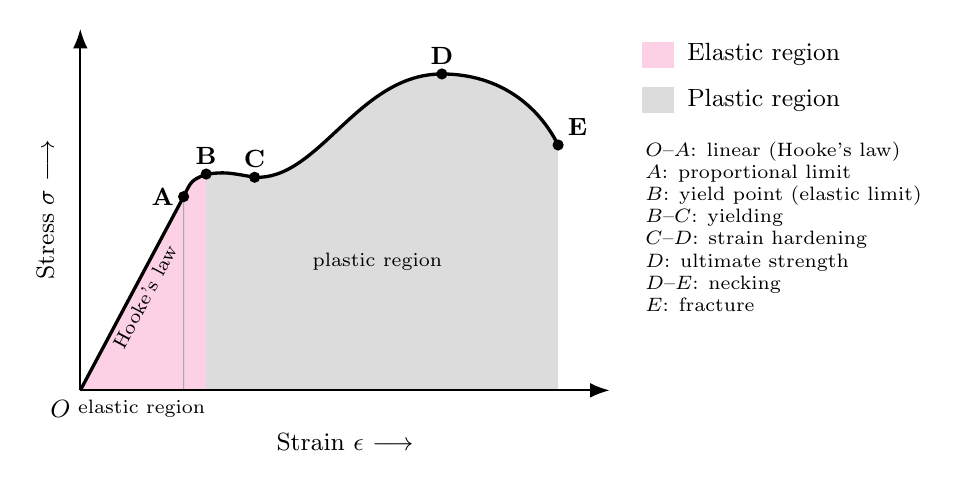
\begin{tikzpicture}[scale=0.82,font=\small]
          \coordinate (O) at (0,0);
          \coordinate (A) at (1.6,3.0);
          \coordinate (B) at (1.95,3.35);
          \coordinate (C) at (2.7,3.3);
          \coordinate (D) at (5.6,4.9);
          \coordinate (E) at (7.4,3.8);
          % shaded regions under the curve
          \fill[RubineRed!18] (O) -- (A) .. controls (1.72,3.25) .. (B) -- (1.95,0) -- cycle;
          \fill[LightGray!80] (1.95,0) -- (B) .. controls (2.25,3.38) .. (C)
               .. controls (3.7,3.25) and (4.3,4.9) .. (D)
               .. controls (6.5,4.9) and (7.1,4.4) .. (E) -- (7.4,0) -- cycle;
          \draw[DarkGray] (A) -- (1.6,0);
          % axes
          \draw[-{Latex[length=2.5mm]},thick] (0,0) -- (8.2,0);
          \draw[-{Latex[length=2.5mm]},thick] (0,0) -- (0,5.6);
          \node[below=12pt] at (4.1,0) {Strain $\epsilon$ $\longrightarrow$};
          \node[rotate=90,above=6pt] at (0,2.8) {Stress $\sigma$ $\longrightarrow$};
          \node[below left] at (O) {$O$};
          % curve
          \draw[very thick] (O) -- (A) .. controls (1.72,3.25) .. (B) .. controls (2.25,3.38) .. (C)
               .. controls (3.7,3.25) and (4.3,4.9) .. (D)
               .. controls (6.5,4.9) and (7.1,4.4) .. (E);
          \foreach \p/\pos in {A/left,B/above,C/above,D/above,E/above right}{
            \filldraw (\p) circle (2.2pt);
            \node[\pos] at (\p) {\textbf{\p}};
          }
          \node[rotate=62] at (1.0,1.45) {\scriptsize Hooke's law};
          \node[below] at (0.95,0) {\scriptsize elastic region};
          \node at (4.6,2.0) {\scriptsize plastic region};
          % legend
          \fill[RubineRed!18] (8.7,5.0) rectangle (9.2,5.4);
          \node[right] at (9.25,5.2) {Elastic region};
          \fill[LightGray!80] (8.7,4.3) rectangle (9.2,4.7);
          \node[right] at (9.25,4.5) {Plastic region};
          \node[anchor=north west,align=left,font=\scriptsize] at (8.6,4.0) {$O$--$A$: linear (Hooke's law)\\ $A$: proportional limit\\ $B$: yield point (elastic limit)\\ $B$--$C$: yielding\\ $C$--$D$: strain hardening\\ $D$: ultimate strength\\ $D$--$E$: necking\\ $E$: fracture};
        \end{tikzpicture}
        \caption{Stress vs. Strain.
        Note that the linear part of the graph represents a Hookean material that follows Hooke's law. The plastic region is the area on a stress-strain curve that represents the material's behavior after it has yielded.}
    \end{figure}
    \vspace{-3mm}
    {\centering\tiny\color{DarkGray}Schematic: instructor's course notes (redrawn; qualitative curve for a ductile metal).\par}
\end{frame}

\begin{frame}{Multidimensional Stress and Strain}
    \begin{itemize}
        \item Real-world problems often involve multidimensional loading and deformation, beyond the 1D case.
        \item In higher dimensions, stress and strain become tensor quantities, with both magnitude and multiple directions.
        \item This complexity arises from forces acting on a body in various directions, causing deformation in multiple ways.
        \item Stress and strain tensors are needed to fully describe the state of stress and strain in multidimensional settings.
        \item These tensors capture the complex interplay of forces and deformations, providing a complete picture of material behavior.
    \end{itemize}
\end{frame}

\begin{frame}{Types of Stress}
  \begin{itemize}
    \item \textbf{Tensile Stress:} Stretching (e.g., ligament under tension).
    \item \textbf{Compressive Stress:} Squeezing (e.g., bone under load).
    \item \textbf{Shear Stress:} Tangential force (e.g., sliding of tissue layers).
  \end{itemize}
\end{frame}

\begin{frame}{Loading Definitions}
Loading refers to the application of external forces or moments to a solid body. These applied forces and moments cause internal stresses and strains within the material, which can lead to deformation or even failure.
  \begin{itemize}
    \item \textbf{Axial Loading:} Force along the longitudinal axis (tensile or compressive).
    \item \textbf{Bending:} Application of a moment, inducing tensile and compressive stresses. Moment: $M=Fd$
    \item \textbf{Torsion:} Twisting, inducing shear stress. Torque: $T=Fr$
  \end{itemize}
\end{frame}

\begin{frame}{Supporting Image}
    \begin{figure}
        % Native redraw of ../pictures/2-1/Moment-Torque.png (PNG kept on disk; the AI-generated
        % original contained the garbled label "(Force along long.Fe)").
        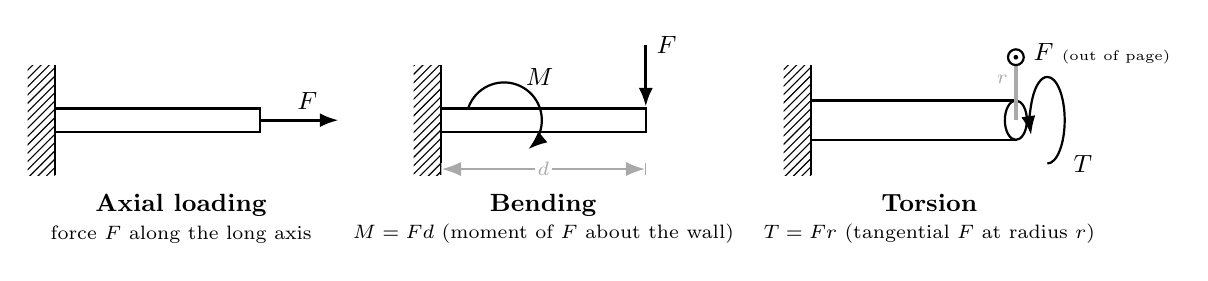
\begin{tikzpicture}[font=\small,>={Latex[length=2.4mm]}]
          % ---- panel 1: axial loading ----
          \begin{scope}[shift={(0,0)}]
            \fill[pattern=north east lines] (-0.35,-0.7) rectangle (0,0.7);
            \draw[thick] (0,-0.7) -- (0,0.7);
            \draw[thick,fill=white] (0,-0.15) rectangle (2.6,0.15);
            \draw[->,very thick] (2.6,0) -- (3.6,0) node[pos=0.6,above] {$F$};
            \node[align=center] at (1.6,-1.25) {\textbf{Axial loading}\\[-1pt] \scriptsize force $F$ along the long axis};
          \end{scope}
          % ---- panel 2: bending ----
          \begin{scope}[shift={(4.9,0)}]
            \fill[pattern=north east lines] (-0.35,-0.7) rectangle (0,0.7);
            \draw[thick] (0,-0.7) -- (0,0.7);
            \draw[thick,fill=white] (0,-0.15) rectangle (2.6,0.15);
            \draw[->,very thick] (2.6,0.95) -- (2.6,0.17) node[pos=0,right] {$F$};
            \draw[|<->|,DarkGray] (0,-0.62) -- (2.6,-0.62) node[midway,fill=white,inner sep=1pt] {\scriptsize $d$};
            \draw[->,thick] ([shift={(160:0.48)}]0.8,0) arc[start angle=160,end angle=-50,radius=0.48];
            \node at (1.25,0.55) {$M$};
            \node[align=center] at (1.3,-1.25) {\textbf{Bending}\\[-1pt] \scriptsize $M = Fd$ (moment of $F$ about the wall)};
          \end{scope}
          % ---- panel 3: torsion ----
          \begin{scope}[shift={(9.6,0)}]
            \fill[pattern=north east lines] (-0.35,-0.7) rectangle (0,0.7);
            \draw[thick] (0,-0.7) -- (0,0.7);
            \draw[thick,fill=white] (0,-0.25) rectangle (2.6,0.25);
            \draw[thick,fill=white] (2.6,0) ellipse (0.14 and 0.25);
            \draw[very thick,DarkGray] (2.6,0) -- (2.6,0.8) node[pos=0.65,left=-1pt] {\scriptsize $r$};
            \draw[thick,fill=white] (2.6,0.8) circle (0.1);
            \fill (2.6,0.8) circle (0.03);
            \node[right,align=left] at (2.7,0.85) {$F$ \tiny(out of page)};
            \draw[->,thick] (3.0,-0.55) arc[start angle=-90,end angle=200,x radius=0.22,y radius=0.55];
            \node at (3.45,-0.55) {$T$};
            \node[align=center] at (1.5,-1.25) {\textbf{Torsion}\\[-1pt] \scriptsize $T = Fr$ (tangential $F$ at radius $r$)};
          \end{scope}
        \end{tikzpicture}
        \caption{An image of a rod fixed at one end and subjected to an axial loading, bending with moment $M$, and torque $T$.}
    \end{figure}
    \vspace{-3mm}
    {\centering\tiny\color{DarkGray}Schematic: instructor's course notes.\par}
\end{frame}

\begin{frame}{Material Properties: Young's Modulus}
  \begin{itemize}
    \item \textbf{Young's Modulus (E):} Stiffness of a material.
      \begin{itemize}
        \item $\sigma = E\epsilon$ (Linear elastic region)
        \item High E: Stiff material (e.g., cortical bone).
        \item Low E: Flexible material (e.g., soft tissue).
      \end{itemize}
  \end{itemize}
\end{frame}

\begin{frame}{Material Properties: Poisson's Ratio}
  \begin{itemize}
    \item \textbf{Poisson's Ratio ($\nu$):} Ratio of lateral to axial strain.
      \begin{itemize}
        \item $\nu = -\frac{\epsilon_{lateral}}{\epsilon_{axial}}$
        \item The minus sign makes $\nu$ positive for ordinary materials: stretching ($\epsilon_{axial}>0$) makes the bar thinner ($\epsilon_{lateral}<0$).
        \item Affects volume changes under load: for small strains the volume change in a uniaxial test is $\Delta V/V \approx (1-2\nu)\,\epsilon_{axial}$, which vanishes when $\nu = 1/2$.
      \end{itemize}
  \end{itemize}
      \begin{figure}
        % Native redraw of ../pictures/2-1/poisson.png (PNG kept on disk; the original
        % formula omitted the minus sign).
        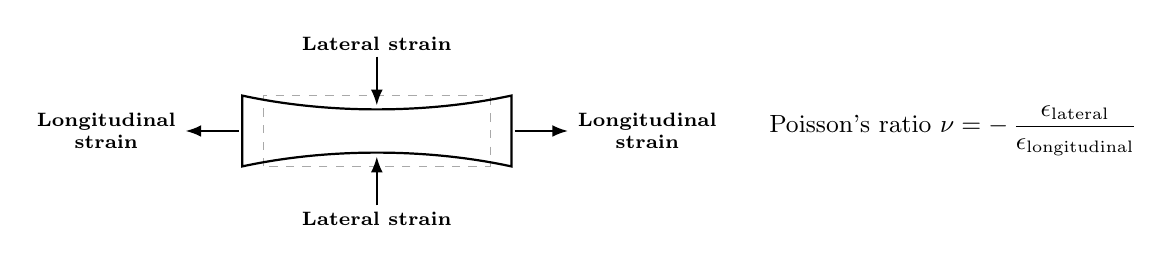
\begin{tikzpicture}[font=\scriptsize,>={Latex[length=2mm]},scale=0.9]
          \draw[dashed,DarkGray] (-1.6,-0.5) rectangle (1.6,0.5);
          \draw[thick] (-1.9,0.5) .. controls (-0.7,0.24) and (0.7,0.24) .. (1.9,0.5)
                       -- (1.9,-0.5) .. controls (0.7,-0.24) and (-0.7,-0.24) .. (-1.9,-0.5) -- cycle;
          \draw[->,thick] (-1.95,0) -- (-2.7,0);
          \draw[->,thick] (1.95,0) -- (2.7,0);
          \node[left,align=center] at (-2.7,0) {\textbf{Longitudinal}\\ \textbf{strain}};
          \node[right,align=center] at (2.7,0) {\textbf{Longitudinal}\\ \textbf{strain}};
          \draw[->,thick] (0,1.05) -- (0,0.36);
          \draw[->,thick] (0,-1.05) -- (0,-0.36);
          \node[above,align=center] at (0,1.0) {\textbf{Lateral strain}};
          \node[below,align=center] at (0,-1.0) {\textbf{Lateral strain}};
          \node[right] at (5.4,0) {\small $\displaystyle \text{Poisson's ratio } \nu = -\,\frac{\epsilon_{\text{lateral}}}{\epsilon_{\text{longitudinal}}}$};
        \end{tikzpicture}
    \end{figure}
    \vspace{-3mm}
    {\centering\tiny\color{DarkGray}Schematic: instructor's course notes (dashed: undeformed shape; solid: stretched shape, exaggerated).\par}
\end{frame}

\begin{frame}{Relating the elastic constants}
  \begin{itemize}
    \item For an isotropic linear elastic solid, only two constants are independent. Given $E$ and $\nu$:
      \begin{align*}
        G = \mu &= \frac{E}{2(1+\nu)} \quad \text{(shear modulus)}\\
        \lambda &= \frac{E\nu}{(1+\nu)(1-2\nu)} \quad \text{(first Lam\'e parameter)}\\
        K &= \frac{E}{3(1-2\nu)} = \lambda + \frac{2\mu}{3} \quad \text{(bulk modulus)}
      \end{align*}
    \item Thermodynamic stability (positive strain energy) requires $-1 < \nu < 1/2$.
    \item $\nu \to 1/2$ is the incompressible limit: $K \to \infty$ and $\lambda \to \infty$, while $\mu$ stays finite.
    \item Soft biological tissue is often modeled as nearly incompressible, with $\nu \approx 0.45$--$0.4999$.
  \end{itemize}
\end{frame}

\begin{frame}{Relating the elastic constants (continued)}
  \begin{itemize}
    \item Conversely, given the Lam\'e parameters $\lambda$ and $\mu$:
      \[
        E = \frac{\mu(3\lambda+2\mu)}{\lambda+\mu}, \qquad
        \nu = \frac{\lambda}{2(\lambda+\mu)} .
      \]
    \item Why the bounds on $\nu$: positive strain energy for every small strain requires $\mu > 0$ and $K > 0$. With $E>0$,
      $\mu = E/[2(1+\nu)] > 0$ gives $\nu > -1$, and $K = E/[3(1-2\nu)] > 0$ gives $\nu < 1/2$.
    \item Most engineering materials have $0 < \nu < 1/2$ (steel $\approx 0.3$, rubber $\approx 0.4999$); materials with $\nu < 0$ (auxetic foams and lattices) are allowed but unusual.
    \item As $\nu \to 1/2$ with $E$ fixed, $\mu \to E/3$. This is why IBFE models of nearly incompressible tissue specify $\mu$ (or a strain-energy function) together with a separate volumetric penalty or bulk modulus, rather than $E$ and $\nu$.
  \end{itemize}
  \vspace{2mm}
  {\tiny\color{DarkGray}Relations as in Bower (2010), \S3.2; Gurtin, Fried \& Anand (2010), part on linear elasticity.\par}
\end{frame}

\begin{frame}{Material Properties: Yield Strength}
  \begin{itemize}
    \item \textbf{Yield Strength ($\sigma_y$):} Stress at which permanent deformation occurs (important for implant design).
    \item When there is no sharp yield point it is defined by the \emph{0.2\% offset} rule: the stress at which unloading would leave a permanent strain of 0.002.
  \end{itemize}
        \begin{figure}
        % Native redraw of ../pictures/2-1/yield-strength.png (PNG kept on disk; original source unknown).
        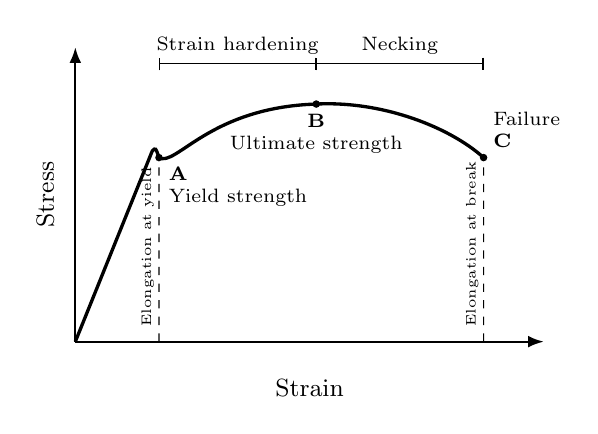
\begin{tikzpicture}[font=\scriptsize,scale=0.85,>={Latex[length=2mm]}]
          \draw[->,thick] (0,0) -- (7.0,0) node[midway,below=10pt] {\small Strain};
          \draw[->,thick] (0,0) -- (0,4.4) node[midway,rotate=90,above=4pt] {\small Stress};
          \coordinate (A) at (1.25,2.75);
          \coordinate (B) at (3.6,3.55);
          \coordinate (C) at (6.1,2.75);
          \draw[very thick] (0,0) -- (1.15,2.85) .. controls (1.2,2.9) .. (A)
                .. controls (1.5,2.6) and (2.0,3.5) .. (B)
                .. controls (4.6,3.6) and (5.6,3.2) .. (C);
          \fill (A) circle (1.6pt); \fill (B) circle (1.6pt); \fill (C) circle (1.6pt);
          \node[below right,align=left] at (A) {\textbf{A}\\ Yield strength};
          \node[below,align=center] at (B) {\textbf{B}\\ Ultimate strength};
          \node[above right,align=left] at (C) {Failure\\ \textbf{C}};
          \draw[dashed] (1.25,0) -- (A);
          \draw[dashed] (6.1,0) -- (C);
          \node[rotate=90,anchor=west,font=\tiny] at (1.08,0.08) {Elongation at yield};
          \node[rotate=90,anchor=west,font=\tiny] at (5.93,0.08) {Elongation at break};
          \draw[|-|] (1.25,4.15) -- (3.6,4.15) node[midway,above] {Strain hardening};
          \draw[|-|] (3.6,4.15) -- (6.1,4.15) node[midway,above] {Necking};
        \end{tikzpicture}
    \end{figure}
    \vspace{-3mm}
    {\centering\tiny\color{DarkGray}Schematic: instructor's course notes (redrawn; qualitative curve for a ductile material).\par}
\end{frame}

\begin{frame}{Material Behavior}
  \begin{itemize}
    \item \textbf{Linear Elastic:} Stress proportional to strain. (Example - steel, aluminum)
    \item \textbf{Non-linear:} Stress-strain relationship is not linear. (Example - Rubber)
    \item \textbf{Viscoelastic:} Time-dependent deformation (creep and relaxation, common in biological tissues)
  \end{itemize}
\end{frame}

\begin{frame}{Pressure and Traction}
  \begin{itemize}
    \item \textbf{Pressure:} Normal force applied over a surface area, acting perpendicular to the surface. $P = \frac{F_n}{A}$ (Pascals). Example: Fluid pressure on tissue.
    \item \textbf{Traction:} Force per unit area acting on a surface, with normal and tangential components (frictional forces). Example: Shear forces between tissue layers.
    \item \textbf{Key Difference:} Pressure is always normal, while traction can have both normal and tangential components.
    \item \textbf{Sign convention:} pressure is taken positive in compression, so a pressure $p$ acting on a surface with \emph{outward} unit normal $\mathbf{n}$ exerts the traction $\mathbf{t} = -p\,\mathbf{n}$ (it pushes inward). In general $\mathbf{t} = \boldsymbol{\sigma}\mathbf{n}$ (deck 2-2).
  \end{itemize}
\end{frame}

\begin{frame}{Boundary Conditions and Loading}
  \begin{itemize}
    \item \textbf{Types of Mechanical Loads:}
      \begin{enumerate}
        \item Prescribed displacements or motion.
        \item Pressure or traction on boundaries.
        \item Mixed displacement and traction.
        \item Body forces (gravity, electromagnetic).
        \item Contact between solids (or self-contact).
        \item Thermal or material process-induced stresses.
      \end{enumerate}
    \item Items 1--3 and 5 are \emph{boundary} conditions; items 4 and 6 act throughout the volume and enter the field equations (body force $\mathbf{b}$, thermal or residual strain) rather than the boundary data.
  \end{itemize}
  \vspace{2mm}
  {\tiny\color{DarkGray}Adapted from Bower (2010), Ch.~1 (defining a problem in solid mechanics: loading and boundary conditions).\par}
\end{frame}

\begin{frame}{Boundary Condition Rules}
  \begin{itemize}
    \item \textbf{3D:} 3 components of displacement or traction at each boundary point. For each of the three directions, exactly one of the conjugate pair (displacement component $u_i$ \emph{or} traction component $t_i$) is prescribed; different directions may use different choices.
    \item \textbf{2D:} 2 components of displacement or traction at each boundary point.
    \item Static problems with traction only: The resultant force \emph{and} the resultant moment of all applied tractions and body forces must vanish,
      \[
        \int_{\partial V} \mathbf{t}\,dA + \int_V \mathbf{b}\,dV = \mathbf{0}, \qquad
        \int_{\partial V} \mathbf{x}\times\mathbf{t}\,dA + \int_V \mathbf{x}\times\mathbf{b}\,dV = \mathbf{0}.
      \]
    \item Even then, the displacement is determined only up to a rigid-body motion (translation plus infinitesimal rotation), which must be fixed by extra constraints.
    \item Example (mixed condition): a \emph{roller} support on the plane $x_2 = 0$ prescribes the normal displacement $u_2 = 0$ together with zero tangential tractions $t_1 = t_3 = 0$ (frictionless sliding).
  \end{itemize}
  \vspace{1mm}
  {\tiny\color{DarkGray}Adapted from Bower (2010), Ch.~1 (loading and boundary conditions).\par}
\end{frame}

\begin{frame}{Boundary Conditions: Practical Considerations}
  \begin{itemize}
    \item Loading can be complex (earthquakes, wind, contact).
    \item Requires accurate estimation of loading parameters (acceleration, pressure, friction).
    \item Nano-scale or biological applications: Consider attractive forces.
    \item In IBFE the dominant ``loading'' on an immersed structure is usually the fluid itself: fluid stresses act on the structure through the coupled momentum equation rather than as a prescribed traction.
  \end{itemize}
  \vspace{2mm}
  {\tiny\color{DarkGray}Adapted from Bower (2010), Ch.~1 (loading and boundary conditions).\par}
\end{frame}

\begin{frame}{Material Models}
    \begin{itemize}
        \item \textbf{Isotropic Linear Elasticity:} Material properties are the same in all directions. $\sigma_{ij} = C_{ijkl}\,\varepsilon_{kl}$ (fourth-order stiffness tensor; 2 independent constants for isotropy), simplified to $\sigma = E \epsilon$ (1D).
        \item \textbf{Anisotropic Linear Elasticity:} Material properties vary with direction (e.g., bone). Requires a full stiffness tensor.
        \item \textbf{Hyperelasticity:} Large deformations, non-linear elastic behavior. Strain energy function $W(\epsilon)$ describes the material response (e.g., soft tissues). (For finite strain, $W$ is written in terms of the deformation gradient, $W(\mathbf{F})$ or $W(\mathbf{C})$ with $\mathbf{C}=\mathbf{F}^T\mathbf{F}$, rather than the small strain $\epsilon$; see deck 4-2.)
        \item \textbf{Viscoelasticity:} Time-dependent deformation. Stress depends on strain rate. Generalized Maxwell or Kelvin-Voigt models. $\sigma(t) = \int_{-\infty}^{t} G(t-\tau) \frac{d\epsilon(\tau)}{d\tau} d\tau$, where $G$ is the stress-relaxation modulus.
        \item \textbf{Viscoplasticity:} Time-dependent plastic (permanent) deformation. Yield stress depends on strain rate (e.g., metals at high temperature, polymers; bone shows rate-dependent post-yield behavior). (Bone \emph{remodeling} is a slower biological adaptation, usually modeled separately.)
    \end{itemize}
\end{frame}

\begin{frame}{Isotropic Linear Elasticity in Tensor Form}
  \begin{itemize}
    \item For an isotropic material the fourth-order stiffness tensor reduces to two constants, and $\sigma_{ij} = C_{ijkl}\,\varepsilon_{kl}$ becomes
      \[
        \sigma_{ij} = \lambda\,\varepsilon_{kk}\,\delta_{ij} + 2\mu\,\varepsilon_{ij},
        \qquad
        \varepsilon_{ij} = \tfrac12\left(\frac{\partial u_i}{\partial x_j} + \frac{\partial u_j}{\partial x_i}\right),
      \]
      i.e.\ $C_{ijkl} = \lambda\,\delta_{ij}\delta_{kl} + \mu(\delta_{ik}\delta_{jl} + \delta_{il}\delta_{jk})$ (summation over repeated indices).
    \item Equivalently, in terms of $E$ and $\nu$:
      \(
        \varepsilon_{ij} = \frac{1+\nu}{E}\,\sigma_{ij} - \frac{\nu}{E}\,\sigma_{kk}\,\delta_{ij}.
      \)
    \item Check in 1D: a uniaxial stress $\sigma_{11}=\sigma$, all other $\sigma_{ij}=0$, gives $\varepsilon_{11} = \sigma/E$ (Hooke's law) and $\varepsilon_{22}=\varepsilon_{33} = -\nu\sigma/E = -\nu\,\varepsilon_{11}$ (Poisson's ratio).
    \item A general anisotropic $C_{ijkl}$ has at most 21 independent constants (after using the symmetries of $\sigma$, $\varepsilon$ and the existence of a strain energy).
  \end{itemize}
  \vspace{1mm}
  {\tiny\color{DarkGray}After Bower (2010), \S3.2.\par}
\end{frame}

\begin{frame}{Equations of Motion for an Elastic Body}
  \begin{itemize}
    \item Apply \textbf{balance of linear momentum} (Newton's second law) to an arbitrary material volume $V$ with surface $\partial V$:
      \[
        \frac{d}{dt}\int_V \rho\,\mathbf{v}\,dV = \int_{\partial V} \mathbf{t}\,dA + \int_V \mathbf{b}\,dV ,
        \qquad \mathbf{t} = \boldsymbol{\sigma}\mathbf{n},
      \]
      where $\mathbf{b}$ is the body force per unit volume (e.g.\ $\rho\mathbf{g}$).
    \item The divergence theorem turns the surface integral into $\int_V \nabla\cdot\boldsymbol{\sigma}\,dV$; since $V$ is arbitrary, the integrands must agree pointwise. For small deformations ($\mathbf{v} \approx \partial\mathbf{u}/\partial t$):
      \[
        \boxed{\;\rho\,\frac{\partial^2 \mathbf{u}}{\partial t^2} = \nabla\cdot\boldsymbol{\sigma} + \mathbf{b}\;}
        \qquad
        \rho\,\frac{\partial^2 u_i}{\partial t^2} = \frac{\partial \sigma_{ij}}{\partial x_j} + b_i .
      \]
    \item \textbf{Balance of angular momentum} does not give a new equation of motion; it gives the symmetry $\sigma_{ij} = \sigma_{ji}$ (deck 2-2).
    \item Static equilibrium is the special case $\nabla\cdot\boldsymbol{\sigma} + \mathbf{b} = \mathbf{0}$.
  \end{itemize}
  \vspace{1mm}
  {\tiny\color{DarkGray}Ported (with corrections) from the instructor's earlier notes \texttt{OLD-2-Solid-Mechanics.tex}; derivation as in Bower (2010), \S2.3 (equations of motion), and Gurtin, Fried \& Anand (2010).\par}
\end{frame}

\begin{frame}{Equations of Motion for an Elastic Body (continued)}
  \begin{itemize}
    \item Substituting isotropic linear elasticity, $\boldsymbol{\sigma} = \lambda(\nabla\cdot\mathbf{u})\mathbf{I} + \mu\left(\nabla\mathbf{u} + \nabla\mathbf{u}^T\right)$, with constant $\lambda,\mu$ gives the \textbf{Navier--Cauchy equations}
      \[
        \rho\,\frac{\partial^2 \mathbf{u}}{\partial t^2} = (\lambda+\mu)\,\nabla(\nabla\cdot\mathbf{u}) + \mu\,\nabla^2\mathbf{u} + \mathbf{b}.
      \]
      (Use $\nabla\cdot(\nabla\mathbf{u}^T) = \nabla(\nabla\cdot\mathbf{u})$ and $\nabla\cdot(\nabla\mathbf{u}) = \nabla^2\mathbf{u}$.)
    \item These support pressure waves with speed $c_p = \sqrt{(\lambda+2\mu)/\rho}$ and shear waves with speed $c_s = \sqrt{\mu/\rho}$; for nearly incompressible tissue $c_p \gg c_s$, which limits explicit time steps.
    \item For \textbf{large deformations} the same balance law is written on the reference configuration with the first Piola--Kirchhoff stress $\mathbf{P}$:
      \(
        \rho_0\,\frac{\partial^2 \mathbf{u}}{\partial t^2} = \nabla_X\cdot\mathbf{P} + \mathbf{b}_0 ,
      \)
      the form used by the IBFE structure (deck 4-2).
    \item The equations must be supplemented by boundary conditions (previous slides) and initial conditions $\mathbf{u}(\mathbf{x},0)$, $\partial_t\mathbf{u}(\mathbf{x},0)$.
  \end{itemize}
  \vspace{1mm}
  {\tiny\color{DarkGray}After Bower (2010), \S2.3 and Ch.~5 (linear elastic solutions); Holzapfel (2000), Ch.~4.\par}
\end{frame}

\begin{frame}{Applications in Biomaterials}
  \begin{itemize}
    \item Implant design: Matching mechanical properties to host tissue.
    \item Tissue engineering: Understanding cell-matrix interactions.
    \item Biomechanical compatibility: Minimizing stress shielding.
    \item Long-term stability: Predicting implant lifespan.
  \end{itemize}
\end{frame}

\begin{frame}{References}
  \scriptsize
  \begin{itemize}
    \item A. F. Bower, \emph{Applied Mechanics of Solids}, CRC Press, Boca Raton, 2010. doi:10.1201/9781439802489. Online version: \url{https://solidmechanics.org} (Ch.~1, \S2.3, \S3.2, Ch.~5 drawn on here).
    \item M. E. Gurtin, E. Fried, L. Anand, \emph{The Mechanics and Thermodynamics of Continua}, Cambridge University Press, 2010. doi:10.1017/CBO9780511762956.
    \item G. A. Holzapfel, \emph{Nonlinear Solid Mechanics: A Continuum Approach for Engineering}, Wiley, Chichester, 2000.
    \item B. E. Griffith, IBFE lecture (video), \url{https://www.youtube.com/watch?v=-1TlNJL93sc} (solid mechanics from the 23-minute mark).
    \item M. Santiago, \emph{Intro to Solid Mechanics} (course notes, shared folder linked on the Resources slide).
    \item Instructor's earlier notes, \texttt{OLD-2-Solid-Mechanics.tex} (source of the equations-of-motion slides, corrected here).
  \end{itemize}
  \medskip
  \textbf{Figures.} Tensile-rod illustration: generated with AI assistance for these notes. Stress--strain curves, loading modes, and Poisson's-ratio sketch: schematics redrawn for these notes (the earlier raster versions remain in \texttt{pictures/}).

  \medskip
  \textbf{Further reading.} P. A. Kelly, \emph{Solid Mechanics Part I: An Introduction to Solid Mechanics} and \emph{Part III: Foundations of Continuum Solid Mechanics}, lecture notes, University of Auckland (online).
\end{frame}


\end{document}